%to-do: adjust refs.bib to the new folder structure
%to-do: undo the escape characters in the double underscores
%to-do: add a nocite on the table of contents slide such that the paper one is presenting gets cited in the bibliography
\documentclass[11pt]{beamer}

% Packages ====================================================================
\usepackage{arev}
\usepackage[T1]{fontenc}
\usepackage[utf8]{inputenc}
\usepackage{float, afterpage, rotating, graphicx}
\usepackage{epstopdf}
\usepackage{longtable, booktabs, tabularx}
\usepackage{fancyvrb, moreverb, relsize}
\usepackage{eurosym, calc, chngcntr}
\usepackage{amsmath, amssymb, amsfonts, amsthm}
\usepackage{xcolor}
\usepackage{verbatim}
\usepackage{setspace}
\usepackage{appendixnumberbeamer}
\usepackage{subcaption}
\usepackage{ragged2e}
\usepackage[backend=biber, natbib=true, bibencoding=inputenc, bibstyle=authoryear-ibid, citestyle=authoryear-comp, maxcitenames=3, maxbibnames=10]{biblatex}
\setlength{\bibitemsep}{1.5ex}
\addbibresource{../../../refs.bib}
\hypersetup{colorlinks=true, linkcolor=., anchorcolor=., citecolor=., filecolor=., menucolor=., runcolor=., urlcolor=.}

% Commands =====================================================================
\DeclareMathOperator*{\argmin}{arg\,min}
\DeclareMathOperator*{\argmax}{arg\,max}
\renewcommand{\vec}[1]{\mathbf{#1}}
\def\newblock{\hskip .11em plus .33em minus .07em}
\newcommand{\bs}{\boldsymbol}
\newcommand{\N}{\mathbb{N}}
\newcommand{\cov}{\mathrm{cov}\thin}
\newcommand{\thin}{\thinspace}
\newcommand{\thick}{\thickspace}
\newcommand{\Lim}[1]{\raisebox{0.5ex}{\scalebox{0.8}{$\displaystyle \lim_{#1}\;$}}}
\newcommand{\vect}[1]{\mathbf{#1}}
\newcommand{\myfrac}[3][0pt]{\genfrac{}{}{}{}{\raisebox{#1}{$#2$}}{\raisebox{-#1}{$#3$}}}
\newcommand{\U}{\mathrm{U}} %Uniform Distribution
\newcommand{\D}{\mathrm{D}} %Dirichlet Distribution
\newcommand{\W}{\mathrm{W}} %Wishart Distribution
\newcommand{\E}{\mathrm{E}}     %Expectation
\newcommand{\Prob}{\mbox{Pr}}       %Expectation
\newcommand{\Iden}{\mathbb{I}}  %Identity Matrix
\newcommand{\Ind}{\mathrm{I}}   %Indicator Function
\newcommand{\Tau}{\mathcal{T}\thin}
\newcommand{\var}{\mathrm{var}\thin}
\newcommand{\plim}{\mathrm{plim}\thin}
\newcommand\indep{\protect\mathpalette{\protect\independenT}{\perp}}
\def\independenT#1#2{\mathrel{\rlap{$#1#2$}\mkern5mu{#1#2}}}
\newcommand{\notindep}{\ensuremath{\perp\!\!\!\!\!\!\diagup\!\!\!\!\!\!\perp}}%
\newcommand{\mc}{\multicolumn}
\newcommand{\ph}{\phantom}

\newcommand\Wider[2][3em]{%
\makebox[\linewidth][c]{%
  \begin{minipage}{\dimexpr\textwidth+#1\relax}
  \raggedright#2
  \end{minipage}%
  }%
}

% Colors =======================================================================
% short color names
% blues
\definecolor{lb}{HTML}{3498DB}
\definecolor{b}{HTML}{1565C0}
\definecolor{db}{HTML}{002080}
% greens
\definecolor{lg}{HTML}{B2EC5D}
\definecolor{g}{HTML}{55A868}
\definecolor{dg}{HTML}{2E7D32}
% yellows
\definecolor{ly}{HTML}{F9A825}
\definecolor{y}{HTML}{FF8F00}
\definecolor{dy}{HTML}{EF6C00}
% reds
\definecolor{lr}{HTML}{D84315}
\definecolor{r}{HTML}{C44E52}
\definecolor{dr}{HTML}{C62828}
% violet
\definecolor{lv}{HTML}{C71585}
\definecolor{v}{HTML}{9B59B6}
\definecolor{dv}{HTML}{6A1B9A}
% grey
\definecolor{ln}{HTML}{BDBDBD}
\definecolor{n}{HTML}{757575}
\definecolor{dn}{HTML}{616161}
% palettes
\definecolor{p1}{HTML}{4A6FAC}
\definecolor{p2}{HTML}{53A465}
\definecolor{p3}{HTML}{C04C50}
\definecolor{p4}{HTML}{7E6FAE}
\definecolor{p5}{HTML}{C8B571}
\definecolor{p6}{HTML}{62B1C8}
% brown
\definecolor{brown}{HTML}{4E342E}

% long color names
\definecolor{mm-lightblue}{HTML}{3498DB}
\definecolor{md-lightblue}{HTML}{0277BD}
\definecolor{mm-blue}{HTML}{002080}
\definecolor{md-blue}{HTML}{1565C0}
\definecolor{md-indigo}{HTML}{283593}

\definecolor{md-lime}{HTML}{9E9D24}
\definecolor{mm-lightgreen}{HTML}{B2EC5D}
\definecolor{md-lightgreen}{HTML}{558B2F}
\definecolor{mm-green}{HTML}{55A868}
\definecolor{md-green}{HTML}{2E7D32}
\definecolor{md-teal}{HTML}{00695C}

\definecolor{md-yellow}{HTML}{F9A825}
\definecolor{mm-gold}{HTML}{FFBF00}
\definecolor{md-amber}{HTML}{FF8F00}
\definecolor{md-orange}{HTML}{EF6C00}
\definecolor{md-deeporange}{HTML}{D84315}

\definecolor{mm-red}{HTML}{C44E52}
\definecolor{md-red}{HTML}{C62828}
\definecolor{violetred}{HTML}{C71585}

\definecolor{md-brown}{HTML}{4E342E}

\definecolor{md-pink}{HTML}{AD1457}
\definecolor{mm-violet}{HTML}{9B59B6}
\definecolor{md-purple}{HTML}{6A1B9A}
\definecolor{md-deeppurple}{HTML}{4527A0}

\definecolor{md-lightgrey}{HTML}{BDBDBD}
\definecolor{mm-gray}{HTML}{95A5A6}
\definecolor{md-grey}{HTML}{757575}
\definecolor{md-bluegrey}{HTML}{37474F}
\definecolor{md-darkgrey}{HTML}{616161}

\definecolor{sns-blue}{HTML}{4A6FAC}
\definecolor{sns-green}{HTML}{53A465}
\definecolor{sns-red}{HTML}{C04C50}
\definecolor{sns-violett}{HTML}{7E6FAE}
\definecolor{sns-beige}{HTML}{C8B571}
\definecolor{sns-lightblue}{HTML}{62B1C8}

\definecolor{mediumelectricblue}{rgb}{0.01, 0.31, 0.59}

% Design =======================================================================
% Here you define the main color of the presentation titles and structure elements
\colorlet{theme_color}{mediumelectricblue}
\setbeamertemplate{footline}[frame number]
\setbeamertemplate{navigation symbols}{}
\setbeamertemplate{frametitle}{\centering\vspace{1ex}\insertframetitle\par}
\setbeamerfont{alerted text}{series=\bfseries}
\setbeamerfont{title}{series=\bfseries}
\setbeamertemplate{section in toc}[circle]
\setbeamertemplate{subsection in toc}[square]
\setbeamercolor{structure}{fg=theme_color}
\setbeamercolor{alerted text}{use=structure,fg=structure.fg}


% Settings =====================================================================
\setstretch{1.5}
% Set Padding Around Equations
\AtBeginDocument{%
 \abovedisplayskip=-10pt plus 4pt minus 4pt
 \abovedisplayshortskip=0pt plus 3pt
 \belowdisplayskip=-10pt plus 4pt minus 4pt
 \belowdisplayshortskip=0pt plus 3pt
}

% Symbols =================================================================
\def\itemsymbol{$\blacktriangleright$}
\let\svpar\par
\let\svitemize\itemize
\let\svenditemize\enditemize
\let\svitem\item
\let\svcenter\center
\let\svendcenter\endcenter
\let\svcolumn\column
\let\svendcolumn\endcolumn
\def\newitem{\renewcommand\item[1][\itemsymbol]{\vfill\svitem[##1]}}%
\def\newpar{\def\par{\svpar\vfill}}%
\newcommand\stretchon{%
  \newpar%
  \renewcommand\item[1][\itemsymbol]{\svitem[##1]\newitem}%
  \renewenvironment{itemize}%
    {\svitemize}{\svenditemize\newpar\par}%
  \renewenvironment{center}%
    {\svcenter\newpar}{\svendcenter\newpar}%
  \renewenvironment{column}[2]%
    {\svcolumn{##1}\setlength{\parskip}{\columnskip}##2}%
    {\svendcolumn\vspace{\columnskip}}%
}
\usepackage{pifont}
% check mark in green
\newcommand{\cmark}{\textcolor{sns-green}{\ding{51}}}%
% red cross
\newcommand{\xmark}{\textcolor{sns-red}{\ding{55}}}%

% Structure slides==============================================================
\AtBeginSection[]{%
  \begin{frame}[plain, noframenumbering]
    \centering \huge\alert{\insertsection}\par
  \end{frame}}
\AtBeginSubsection[]{
  \begin{frame}[plain, noframenumbering]
    \centering \Large\alert{\insertsubsection}\par
  \end{frame}}

% Title and Author==============================================================
\author[\_\_MyName\_\_]
{
{\bf }}

\begin{document}

\title{Respy}
\date{\today}

\begin{frame}[plain, noframenumbering]
    \maketitle
    \note{~}
\end{frame}


\begin{frame}[c]\frametitle{What's In It for You?}
\begin{itemize}
  \item You can use it as a learning tool
  % to deeply understand an important class of structural econometric models
  \item You can use it for your own work
  \item It can save you months of work!
  \begin{itemize}
    \item Clean and robust solutions to many problems you find in any serious econometric project
    \item Nice interface, refined over years
  \end{itemize}
\end{itemize}
\end{frame}


% Table of contents ============================================================
\begin{frame}[plain, noframenumbering]\frametitle{Outline}
  \hspace{1cm}\begin{minipage}{\textwidth}
    \tableofcontents
  \end{minipage}
\end{frame}




\section{What is Respy?}


\begin{frame}[c]\frametitle{What Is Respy?}
\begin{itemize}
    \item Python program to estimate and simulate a structural model of labor market choices and human capital accumulation
    \item Under the hood: High performance Fortran code
    \item Models are easy to specify, without touching the code
    \item Well tested and used for several papers
\end{itemize}
\end{frame}

\begin{frame}[c]\frametitle{Why Is There No Stata Command for Life-Cycle Models?}
    \begin{itemize}
        \item Stata is too slow
        \item Stata syntax makes it hard to specify complicated models
        \item Every project is different and requires specific computational tricks to become feasible
        \begin{itemize}
            \item You will have to program yourself!
        \end{itemize}
        \item But you don't have to reinvent the wheel
        \item Respy can be a good starting point
    \end{itemize}
\end{frame}


\begin{frame}[c]\frametitle{Why Is Simulation So Important?}
    \begin{itemize}
      \item Learn about the model
      \item Verify correctness of the code
      \item Simulation based estimation methods
      \item One of the main goals of structural estimation is simulation of counterfactual policies
    \end{itemize}
\end{frame}


\begin{frame}[c]\frametitle{Where to Find Respy}
    \alert{Source Code:}
    \begin{itemize}
      \item \url{https://github.com/OpenSourceEconomics/respy/tree/master/respy}
    \end{itemize}
    \alert{Documentation:}
    \begin{itemize}
      \item \url{https://respy.readthedocs.io/en/latest/}
    \end{itemize}
\end{frame}



\section{Quick Tutorial}


\begin{frame}[c, plain, noframenumbering]
    \begin{figure}
      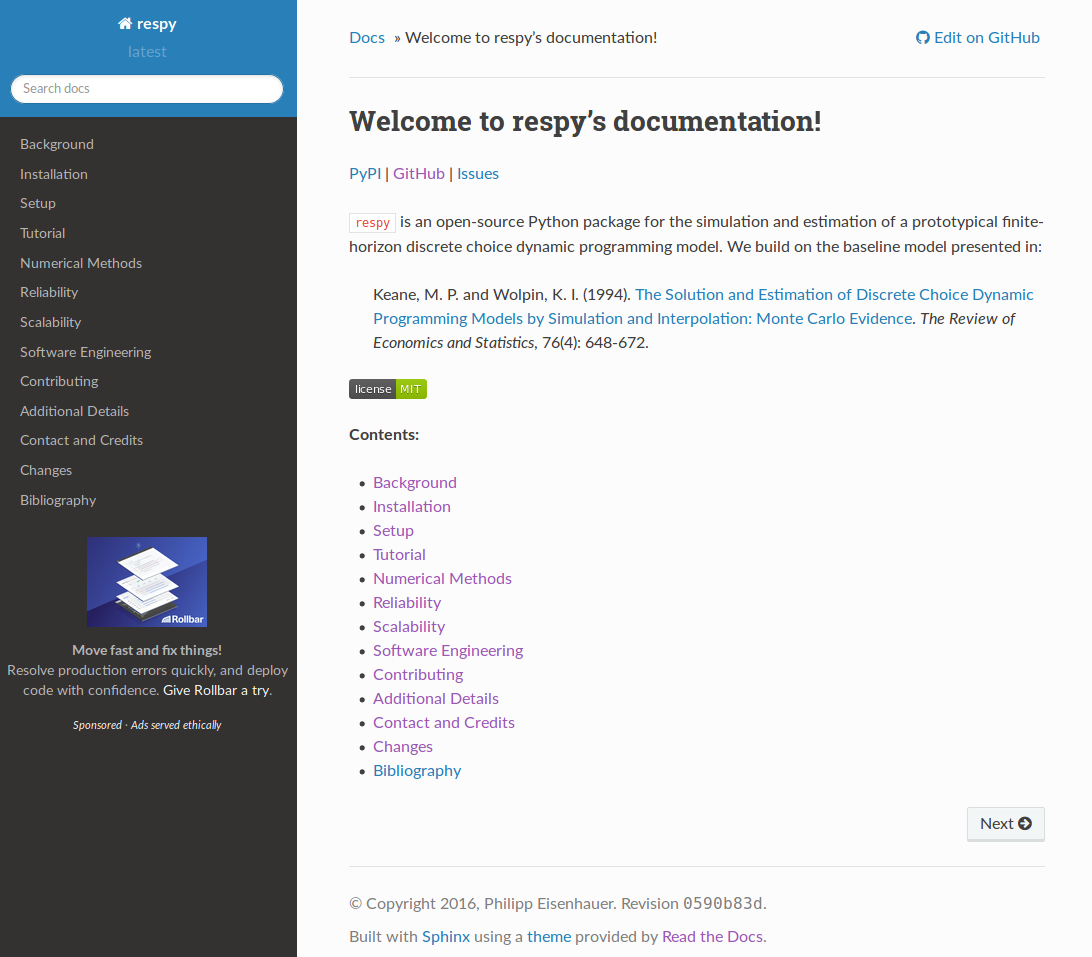
\includegraphics[height=\textheight]{../graphs/respy_rtd.png}
    \end{figure}
\end{frame}




\section{Software Engineering}


\begin{frame}[c]\frametitle{Size of Respy}
    \begin{figure}
      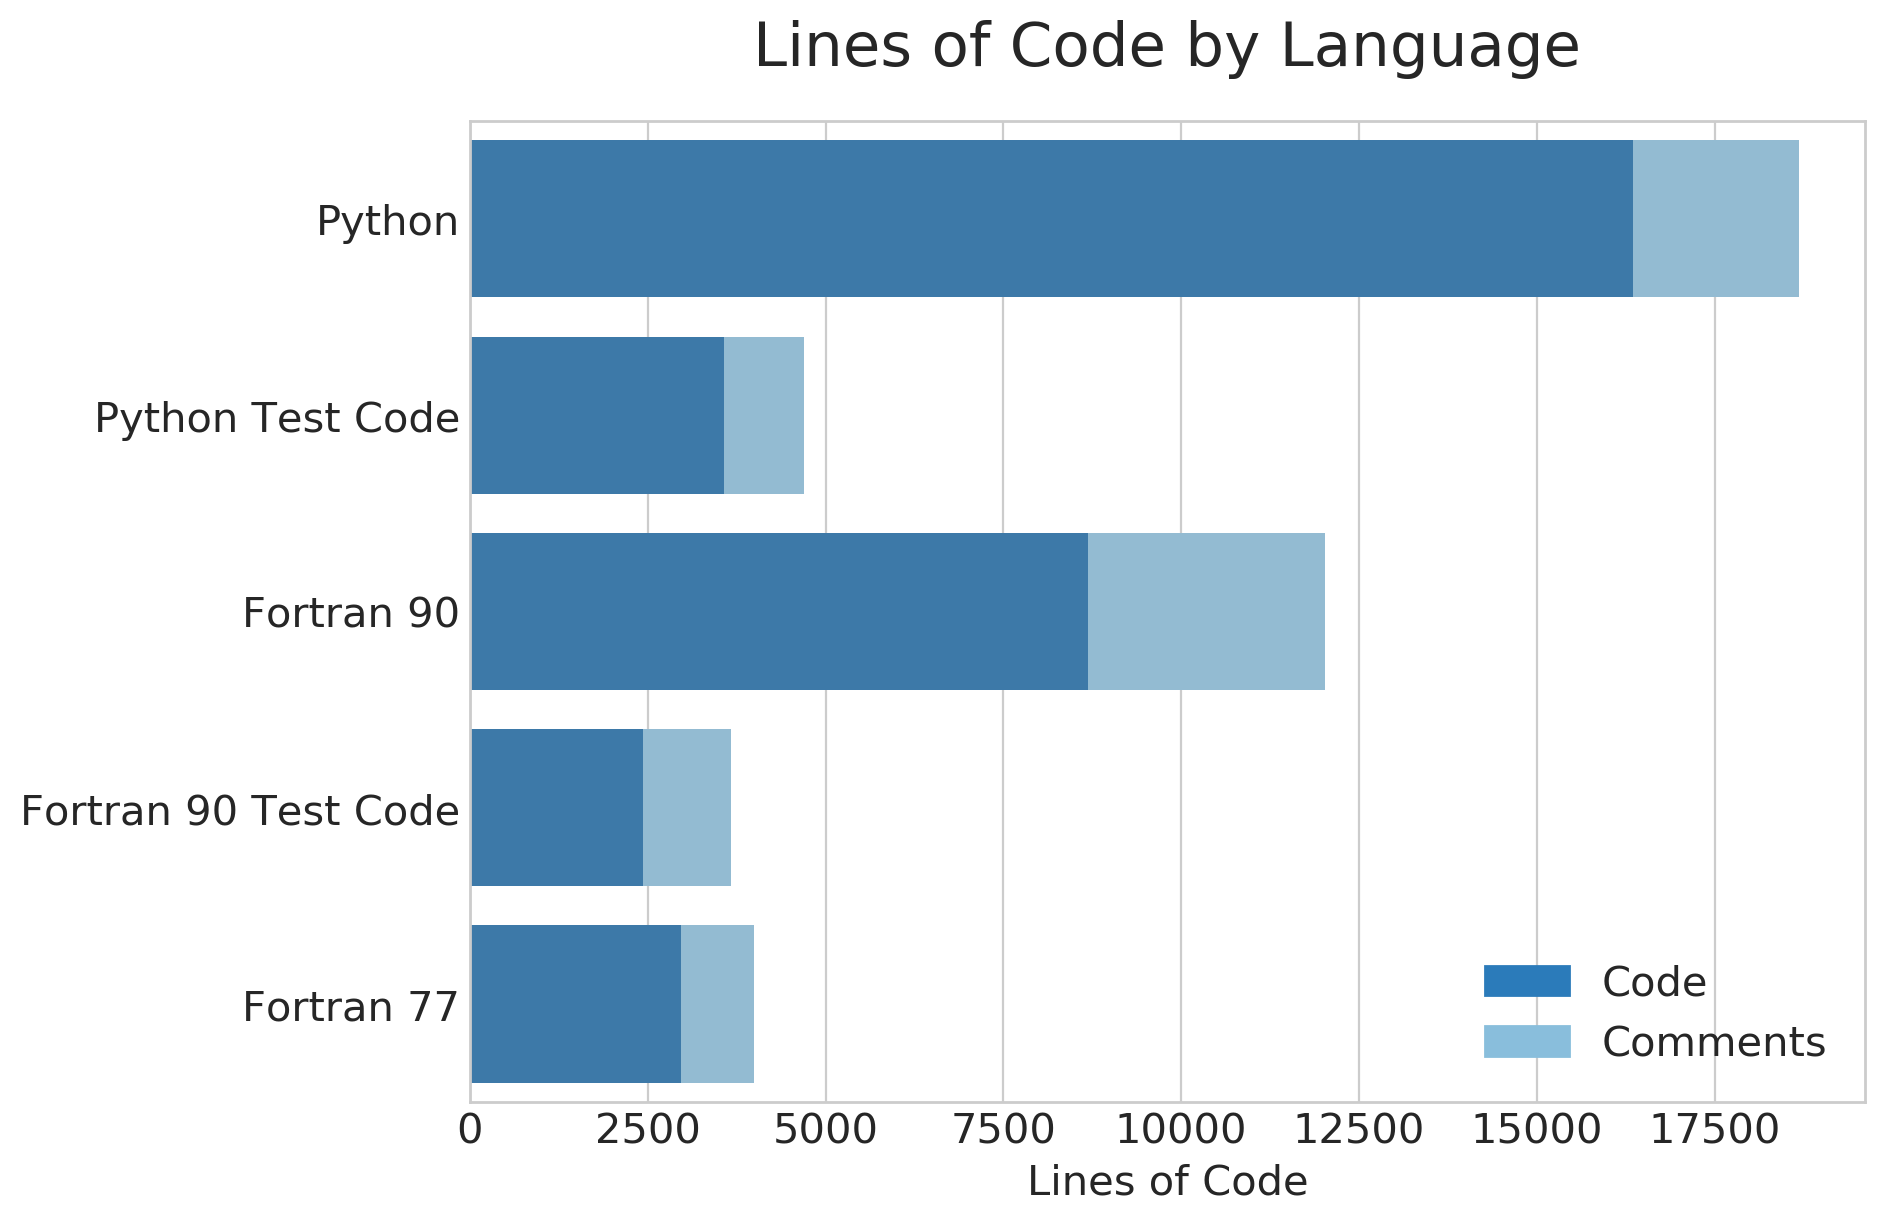
\includegraphics[width=\textwidth]{../../cloc/lines_of_code_by_language.png}
    \end{figure}
\end{frame}

\begin{frame}[c]\frametitle{What is Software Engineering?}
    \begin{itemize}
        \item Strategies to handle complexity and avoid bugs in large software projects
        \item You don't need it if your project consists of one short do-file % but you need it for any serious empirical project

        \item Below, I'll mention two principles; you can find more in the documentation
    \end{itemize}
\end{frame}



\begin{frame}[c]\frametitle{Testing}
\begin{itemize}
  \item Respy has thousands of lines of code
  \item It's easy to introduce a bug \ldots
  \item[] \hspace{2cm} \ldots and hard to find it afterwards!
  \item Thats why we have tests at different levels
  \begin{itemize}
    \item Regression tests
    \item Integration tests
    \item Unit tests
    \item \ldots
  \end{itemize}
\end{itemize}
\end{frame}



\begin{frame}[t]\frametitle{Modularity}
  \begin{itemize}
    \item Respy uses pre-existing code for many tasks
    \begin{itemize}
      \item Numerical optimization
      \item Numerical integration
      \item Linear algebra
    \end{itemize}
    \item Advantages
    \begin{itemize}
      \item Less code to maintain
      \item Highly optimized routines
      \item Easy to switch out parts
    \end{itemize}
  \end{itemize}
\end{frame}



\begin{frame}[c]\frametitle{Modularity II}
\begin{itemize}
    \item The switching out part is extremely important!
    \begin{itemize}
        \item Projects evolve and goals change
        \item At the beginning it's unknown where changes will be
    \end{itemize}
    \item Isolate code for each task even for the code you write yourself!
    \begin{itemize}
        \item Solution, Estimation, \ldots
    \end{itemize}
    \item A well written paper is also modular!
\end{itemize}
\end{frame}









% \appendix
% \begin{frame}[allowframebreaks]
%     \frametitle{References}
%     \renewcommand{\bibfont}{\normalfont\footnotesize}
%     \printbibliography
% \end{frame}

\end{document}


